\chapter{Endogeneity}

    To ensure unbiasedness of OLS estimator, or at least consistency of the OLS estimator we need to have \textit{exogeneity} of the errors, that is
    \begin{align}
        \cov{x,u} = 0
    \end{align}
    The failure of this assumption is called \textit{endogeneity}. Endogeneity can arise for a number of reasons:
    \begin{itemize}
        \item omitted variables
        \item lagged $y$ in the presence of autocorrelation in the error term
        \item simultaneity
        \item measurement errors
    \end{itemize}
    In this chapter we discuss how endogeneity can arise, and several strategies to overcome this.

    \section{Instrumental Variables (IV)}
        
        \subsection{Motivation}

            Suppose we have the following bivariate linear regression model:
            \begin{align}
                y = \beta_0 + \beta_1 x + u
            \end{align}
            If we have endogeneity, i.e. $\cov{x,u} = 0$, then our OLS estimates will be in general, biased. The approach of the previous chapters was to ensure the confounders were appropriately controlled for, and hope $x$ is no longer endogenous. In this section, we introduce another method; through the use of an \textit{instrumental variable} to deal with the endogenous regressor.
            \begin{figure}
                \centering
                
\tikzset{every picture/.style={line width=0.75pt}} %set default line width to 0.75pt        

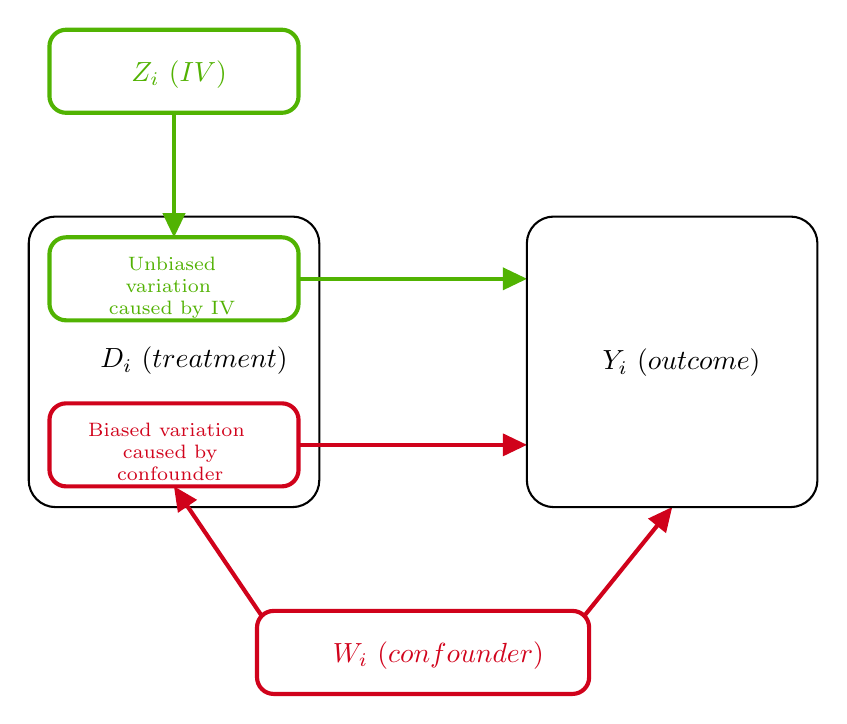
\begin{tikzpicture}[x=0.75pt,y=0.75pt,yscale=-1,xscale=1]
%uncomment if require: \path (0,524); %set diagram left start at 0, and has height of 524

%Rounded Rect [id:dp6497612275953306] 
\draw   (110,203) .. controls (110,195.82) and (115.82,190) .. (123,190) -- (237,190) .. controls (244.18,190) and (250,195.82) .. (250,203) -- (250,317) .. controls (250,324.18) and (244.18,330) .. (237,330) -- (123,330) .. controls (115.82,330) and (110,324.18) .. (110,317) -- cycle ;

%Rounded Rect [id:dp8673780682403747] 
\draw  [color={rgb, 255:red, 81; green, 179; blue, 2 }  ,draw opacity=1 ][line width=1.5]  (120,108) .. controls (120,103.58) and (123.58,100) .. (128,100) -- (232,100) .. controls (236.42,100) and (240,103.58) .. (240,108) -- (240,132) .. controls (240,136.42) and (236.42,140) .. (232,140) -- (128,140) .. controls (123.58,140) and (120,136.42) .. (120,132) -- cycle ;

%Straight Lines [id:da16218237230483512] 
\draw [color={rgb, 255:red, 208; green, 2; blue, 27 }  ,draw opacity=1 ][line width=1.5]    (240,300) -- (346,300) ;
\draw [shift={(350,300)}, rotate = 180] [fill={rgb, 255:red, 208; green, 2; blue, 27 }  ,fill opacity=1 ][line width=0.08]  [draw opacity=0] (11.61,-5.58) -- (0,0) -- (11.61,5.58) -- cycle    ;
%Straight Lines [id:da880895933850384] 
\draw [color={rgb, 255:red, 81; green, 179; blue, 2 }  ,draw opacity=1 ][line width=1.5]    (180,140) -- (180,196) ;
\draw [shift={(180,200)}, rotate = 270] [fill={rgb, 255:red, 81; green, 179; blue, 2 }  ,fill opacity=1 ][line width=0.08]  [draw opacity=0] (11.61,-5.58) -- (0,0) -- (11.61,5.58) -- cycle    ;
%Straight Lines [id:da6515543213351532] 
\draw [color={rgb, 255:red, 81; green, 179; blue, 2 }  ,draw opacity=1 ][line width=1.5]    (240,220) -- (346,220) ;
\draw [shift={(350,220)}, rotate = 180] [fill={rgb, 255:red, 81; green, 179; blue, 2 }  ,fill opacity=1 ][line width=0.08]  [draw opacity=0] (11.61,-5.58) -- (0,0) -- (11.61,5.58) -- cycle    ;
%Rounded Rect [id:dp3607596248065986] 
\draw  [color={rgb, 255:red, 208; green, 2; blue, 27 }  ,draw opacity=1 ][line width=1.5]  (220,388) .. controls (220,383.58) and (223.58,380) .. (228,380) -- (372,380) .. controls (376.42,380) and (380,383.58) .. (380,388) -- (380,412) .. controls (380,416.42) and (376.42,420) .. (372,420) -- (228,420) .. controls (223.58,420) and (220,416.42) .. (220,412) -- cycle ;

%Straight Lines [id:da11780334258026348] 
\draw [color={rgb, 255:red, 208; green, 2; blue, 27 }  ,draw opacity=1 ][line width=1.5]    (222,382) -- (182.24,323.31) ;
\draw [shift={(180,320)}, rotate = 55.89] [fill={rgb, 255:red, 208; green, 2; blue, 27 }  ,fill opacity=1 ][line width=0.08]  [draw opacity=0] (11.61,-5.58) -- (0,0) -- (11.61,5.58) -- cycle    ;
%Straight Lines [id:da6916433454902036] 
\draw [color={rgb, 255:red, 208; green, 2; blue, 27 }  ,draw opacity=1 ][line width=1.5]    (378,382) -- (417.49,333.11) ;
\draw [shift={(420,330)}, rotate = 128.93] [fill={rgb, 255:red, 208; green, 2; blue, 27 }  ,fill opacity=1 ][line width=0.08]  [draw opacity=0] (11.61,-5.58) -- (0,0) -- (11.61,5.58) -- cycle    ;
%Rounded Rect [id:dp8490775320395935] 
\draw  [color={rgb, 255:red, 208; green, 2; blue, 27 }  ,draw opacity=1 ][line width=1.5]  (120,288) .. controls (120,283.58) and (123.58,280) .. (128,280) -- (232,280) .. controls (236.42,280) and (240,283.58) .. (240,288) -- (240,312) .. controls (240,316.42) and (236.42,320) .. (232,320) -- (128,320) .. controls (123.58,320) and (120,316.42) .. (120,312) -- cycle ;

%Rounded Rect [id:dp9976354424664228] 
\draw   (350,203) .. controls (350,195.82) and (355.82,190) .. (363,190) -- (477,190) .. controls (484.18,190) and (490,195.82) .. (490,203) -- (490,317) .. controls (490,324.18) and (484.18,330) .. (477,330) -- (363,330) .. controls (355.82,330) and (350,324.18) .. (350,317) -- cycle ;

%Rounded Rect [id:dp7868826959222632] 
\draw  [color={rgb, 255:red, 81; green, 179; blue, 2 }  ,draw opacity=1 ][line width=1.5]  (120,208) .. controls (120,203.58) and (123.58,200) .. (128,200) -- (232,200) .. controls (236.42,200) and (240,203.58) .. (240,208) -- (240,232) .. controls (240,236.42) and (236.42,240) .. (232,240) -- (128,240) .. controls (123.58,240) and (120,236.42) .. (120,232) -- cycle ;


% Text Node
\draw (135,208) node [anchor=north west][inner sep=0.75pt]  [font=\scriptsize] [align=left] {\begin{minipage}[lt]{63.85pt}\setlength\topsep{0pt}
\begin{center}
\textcolor[rgb]{0.32,0.7,0.01}{Unbiased variation }\\\textcolor[rgb]{0.32,0.7,0.01}{caused by IV}
\end{center}

\end{minipage}};
% Text Node
\draw (128,288) node [anchor=north west][inner sep=0.75pt]  [font=\scriptsize] [align=left] {\begin{minipage}[lt]{72.98pt}\setlength\topsep{0pt}
\begin{center}
\textcolor[rgb]{0.82,0.01,0.11}{Biased variation }\\\textcolor[rgb]{0.82,0.01,0.11}{caused by confounder}
\end{center}

\end{minipage}};
% Text Node
\draw (158,113.4) node [anchor=north west][inner sep=0.75pt]    {$\textcolor[rgb]{0.32,0.7,0.01}{Z_{i} \ \text{(IV)}}$};
% Text Node
\draw (255,393.4) node [anchor=north west][inner sep=0.75pt]    {$\textcolor[rgb]{0.82,0.01,0.11}{W_{i} \ \text{(confounder)}}$};
% Text Node
\draw (385,252.4) node [anchor=north west][inner sep=0.75pt]    {$Y_{i} \ \text{(outcome)}$};
% Text Node
\draw (143,251.4) node [anchor=north west][inner sep=0.75pt]    {$D_{i} \ \text{(treatment)}$};


\end{tikzpicture}
                \caption{Mechanism behind IV}
                \label{fig:IV}
            \end{figure}

            \begin{definition}[IV]
                A valid \textit{instrumental variable}, $z_i$ satisfies two conditions
                \begin{enumerate}
                    \item $z$ is \textbf{exogenous} to the equation, i.e. 
                    \begin{align}
                        \cov{z,u} = 0
                    \end{align}
                    \item $z$ is \textbf{relevant} for explaining $x$, i.e.
                    \begin{align}
                        \cov{z,x} = 0
                    \end{align}
                \end{enumerate}
            \end{definition}

        \subsection{Estimator derivation}
            \begin{theorem}
                If $z$ is an instrumental variable, then $\beta$ can be recovered through
                \begin{align}
                    \beta = \frac{\cov{z,y}}{\cov{z,x}}
                \end{align}
            \end{theorem}
            \begin{proof}
                We have that
                \begin{align}
                    \operatorname{cov}(z,y)= \operatorname{cov}(z,\beta_0 +\beta_1 x +u ) = \beta_1\operatorname{cov}(z, x)
                \end{align}
                Rearrange to yield the result.
            \end{proof}
            \begin{definition}[IV estimator]
                The IV estimator is the MM estimator of $\beta$,
                \begin{align}
                    \hat\beta^\mathrm{IV}_1 = \frac{\ecov{z,y}}{\ecov{z,x}}
                \end{align}
            \end{definition}
            Why is such an instrument beneficial for estimating $\beta_1$? As we know $x$ could be endogenous, this means it is correlated with unknown confounders, as shown in Figure \ref{fig:IV}, and so OLS will produce biased estimates. A valid instrument will allow us to isolate the variation in  uncorrelated with confounders, we call $\hat x_i$, and estimate the effect of $\hat x_i$ on $y_i$, defined as $\hat\beta^\mathrm{IV}_1$ which is a consistent estimate of $\beta_1$ (although it turns out not unbiased).

        \subsection{Wald estimator}\label{def:endogeneity/Wald}
            \begin{definition}
                The \textit{Wald estimator} is defined as
                \begin{align*}
                    \hat\beta_1^\mathrm{Wald} := \frac{\hat\pi_1}{\hat \delta_1}
                \end{align*}
                where $\hat\delta_j$ are the \textit{first stage} regression coefficients,
                \begin{align}
                    x_i = \delta_0 + \delta_1 z_i + e_i 
                \end{align}
                and $\hat\pi_j$ are the \textit{reduced form} coefficients,
                \begin{align}
                    y_i = \pi_0 + \pi_1 z_i + \nu_i
                \end{align}
            \end{definition}
            
            This is equivalent to the IV estimator defined above as
            \begin{align}
                \hat\beta_1^\mathrm{Wald} = \frac{\frac{\ecov{z,y}}{\evar{z}}}{\frac{\ecov{z,x}}{\evar{z_i}}} = \hat\beta^\mathrm{IV}
            \end{align}

        
    \section{Two Stage Least Squares (2SLS)}
    
        IV allows us to overcome selection bias due to endogeneity. 2SLS allows us to generalise IV to binary, count or continuous variables and augment the equation with controls. In addition we can leverage multiple instruments to improve our estimates.

        \subsection{Motivation}
            Let $x$ be our explanatory variable, $y$ is the outcome variable and $z$ is a valid instrument. A baseline regression model would be
            \begin{align}
                y_i = \beta_0 + \beta_1 x_i + u_i
            \end{align}
            However we know that exogeneity fails for $x$, thus OLS is inconsistent and biased.
            
            Recall with \textit{IV/Wald estimators}, we can overcome this by estimating two equations: `First Stage' and `Reduced Form' models
            \begin{align}
                FS:\quad x_i &= \delta_0 + \delta_1 z_i + e_i\\
                RF:\quad y_i &= \pi_0 + \pi_1 z_i + v_i
            \end{align}
            We then compute the ratio as defined in Definition \ref{def:endogeneity/Wald}.

            \textbf{For 2SLS, we proceed as follows.} 
            \begin{enumerate}
                \item First estimate the first stage
                \begin{align}
                    FS:\quad x_i &= \delta_0 + \delta_1 z_i + e_i
                \end{align}
                and obtain predicted values $\hat x_i = \hat\delta_0 + \hat\delta_1 z_i$.
                
                \item Next, we regress $y_i$ on the predicted value of $x_i$, $\hat x_i$,
                \begin{align}
                    y_i = \beta_0^\mathrm{2SLS} + \beta_1^\mathrm{2SLS} \hat x_i + \varepsilon_i
                \end{align}
            \end{enumerate}


        \subsection{Implementation}
            
            \begin{sexylisting}[colback=white, label=lst:endogeneity/2SLS/implement]{2SLS estimation}
//  Run 2SLS regression (robust): 
//  Syntax: outcome control (endog.vars = instruments), robust
ivregress 2sls y w (x_1 x_2 = z_1 z_2 z_3), robust
            \end{sexylisting}
            \noindent It is important to note we \textit{cannot} do:\\ \\
            \indent\verb|reg x_1 z_1 z_2 z_3 w|    \\
            \indent\verb|predict x_1hat|   \\
            \indent\verb|reg x_2 z_1 z_2 z_3 w|    \\
            \indent\verb|predict x_2hat|   \\
            \indent\verb|reg y x_1hat x_2hat w, robust|\\ \\
            This is because when estimating standard error, STATA computes $\hat u_i$ with $\hat x_{j,i}$ instead of $x_{j,i}$ as defined below:
            \begin{align}
                \hat u_i = y_i - \left(\hat\beta_0^\mathrm{2SLS}+\hat\beta_1^\mathrm{2SLS} x_{1,i}+\hat\beta_2^\mathrm{2SLS}  x_{2,i}+\hat\beta_3^\mathrm{2SLS} w_i\right)
            \end{align}
            
        
    \section{Simultaneous Equation Models (SEM)}

        When we investigate demand and supply, we have two simultaneous equations that determine equilibrium quantity and price.
        
        \subsection{Motivation}
            Since we can only observe the black dots where equilibrium occurs, a regression would lead to a misunderstanding of the model, predicted by the black line. Instead what we want to know are the green and red lines, supply and demand equations.

            \begin{figure}
                \centering
                

\tikzset{every picture/.style={line width=0.75pt}} %set default line width to 0.75pt        

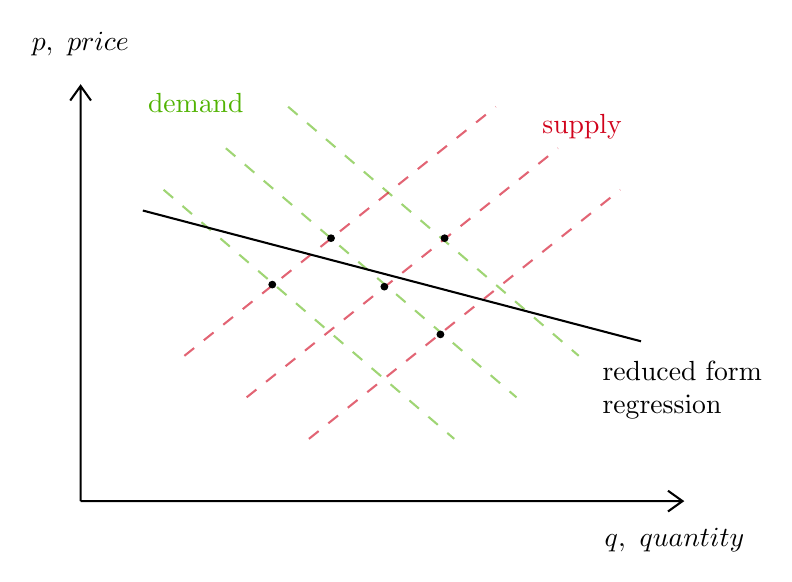
\begin{tikzpicture}[x=0.75pt,y=0.75pt,yscale=-1,xscale=1]
%uncomment if require: \path (0,416); %set diagram left start at 0, and has height of 416

%Shape: Axis 2D [id:dp7232537425646829] 
\draw  (160,270) -- (450,270)(160,70) -- (160,270) -- cycle (443,265) -- (450,270) -- (443,275) (155,77) -- (160,70) -- (165,77)  ;
%Straight Lines [id:da9194583658032972] 
\draw [color={rgb, 255:red, 81; green, 179; blue, 2 }  ,draw opacity=0.55 ] [dash pattern={on 4.5pt off 4.5pt}]  (200,120) -- (340,240) ;
%Straight Lines [id:da09936562819974382] 
\draw [color={rgb, 255:red, 81; green, 179; blue, 2 }  ,draw opacity=0.55 ] [dash pattern={on 4.5pt off 4.5pt}]  (230,100) -- (370,220) ;
%Straight Lines [id:da7284855390717861] 
\draw [color={rgb, 255:red, 81; green, 179; blue, 2 }  ,draw opacity=0.55 ] [dash pattern={on 4.5pt off 4.5pt}]  (260,80) -- (400,200) ;
%Straight Lines [id:da434828806821248] 
\draw [color={rgb, 255:red, 208; green, 2; blue, 27 }  ,draw opacity=0.61 ] [dash pattern={on 4.5pt off 4.5pt}]  (210,200) -- (360,80) ;
%Straight Lines [id:da7067480974690954] 
\draw [color={rgb, 255:red, 208; green, 2; blue, 27 }  ,draw opacity=0.61 ] [dash pattern={on 4.5pt off 4.5pt}]  (240,220) -- (390,100) ;
%Straight Lines [id:da6860399852947346] 
\draw [color={rgb, 255:red, 208; green, 2; blue, 27 }  ,draw opacity=0.61 ] [dash pattern={on 4.5pt off 4.5pt}]  (270,240) -- (420,120) ;
%Flowchart: Connector [id:dp6703726074956241] 
\draw  [fill={rgb, 255:red, 0; green, 0; blue, 0 }  ,fill opacity=1 ] (279.29,143.32) .. controls (279.29,142.59) and (279.89,142) .. (280.64,142) .. controls (281.39,142) and (282,142.59) .. (282,143.32) .. controls (282,144.05) and (281.39,144.64) .. (280.64,144.64) .. controls (279.89,144.64) and (279.29,144.05) .. (279.29,143.32) -- cycle ;
%Flowchart: Connector [id:dp42343723539931355] 
\draw  [fill={rgb, 255:red, 0; green, 0; blue, 0 }  ,fill opacity=1 ] (251,165.68) .. controls (251,164.95) and (251.61,164.36) .. (252.36,164.36) .. controls (253.11,164.36) and (253.71,164.95) .. (253.71,165.68) .. controls (253.71,166.41) and (253.11,167) .. (252.36,167) .. controls (251.61,167) and (251,166.41) .. (251,165.68) -- cycle ;
%Flowchart: Connector [id:dp3602533313351184] 
\draw  [fill={rgb, 255:red, 0; green, 0; blue, 0 }  ,fill opacity=1 ] (305,166.68) .. controls (305,165.95) and (305.61,165.36) .. (306.36,165.36) .. controls (307.11,165.36) and (307.71,165.95) .. (307.71,166.68) .. controls (307.71,167.41) and (307.11,168) .. (306.36,168) .. controls (305.61,168) and (305,167.41) .. (305,166.68) -- cycle ;
%Flowchart: Connector [id:dp5055341802748268] 
\draw  [fill={rgb, 255:red, 0; green, 0; blue, 0 }  ,fill opacity=1 ] (334,143.32) .. controls (334,142.59) and (334.61,142) .. (335.36,142) .. controls (336.11,142) and (336.71,142.59) .. (336.71,143.32) .. controls (336.71,144.05) and (336.11,144.64) .. (335.36,144.64) .. controls (334.61,144.64) and (334,144.05) .. (334,143.32) -- cycle ;
%Flowchart: Connector [id:dp7460489090675402] 
\draw  [fill={rgb, 255:red, 0; green, 0; blue, 0 }  ,fill opacity=1 ] (332,189.68) .. controls (332,188.95) and (332.61,188.36) .. (333.36,188.36) .. controls (334.11,188.36) and (334.71,188.95) .. (334.71,189.68) .. controls (334.71,190.41) and (334.11,191) .. (333.36,191) .. controls (332.61,191) and (332,190.41) .. (332,189.68) -- cycle ;
%Straight Lines [id:da3662864883226279] 
\draw [color={rgb, 255:red, 0; green, 0; blue, 0 }  ,draw opacity=1 ]   (190,130) -- (430,193) ;

% Text Node
\draw (191,72) node [anchor=north west][inner sep=0.75pt]  [color={rgb, 255:red, 81; green, 179; blue, 2 }  ,opacity=1 ] [align=left] {demand};
% Text Node
\draw (381,82) node [anchor=north west][inner sep=0.75pt]  [color={rgb, 255:red, 81; green, 179; blue, 2 }  ,opacity=1 ] [align=left] {\textcolor[rgb]{0.82,0.01,0.11}{supply}};
% Text Node
\draw (410,201) node [anchor=north west][inner sep=0.75pt]   [align=left] {reduced form\\regression};
% Text Node
\draw (135,42.4) node [anchor=north west][inner sep=0.75pt]    {$p,\ \text{price}$};
% Text Node
\draw (411,281.4) node [anchor=north west][inner sep=0.75pt]    {$q,\ \text{quantity}$};


\end{tikzpicture}
                \caption{Simultaneity bias}
                \label{fig:endogeneity/sem}
            \end{figure}

            Now suppose we have the model, or structural equations:
            \begin{align}
                &q_i =\beta_0^{(d)}+\beta_1^{(d)}p_i+e_i^{(d)}\\
                &q_i =\beta_0^{(s)}+\beta_1^{(s)}p_i+e_i^{(s)}
            \end{align}
            We would like to be able to hold one curve constant, while shifting the other, which would allow use to estimate the former, as shown on Figure X. Therefore we need a instrument that will shift one curve and allow us to estimate the other. Let this instrument be denoted $z$, and so our model becomes:
            \begin{align}
                &q_i =\beta_0^{(d)} + \beta_1^{(d)}p_i + e_i^{(d)}\label{eq:endogeneity/demand}\\
                &q_i =\beta_0^{(s)} + \beta_1^{(s)}p_i + \beta_2^{(s)}z^{(s)}_i + e_i^{(s)}\label{eq:endogeneity/supply_w_IV}
            \end{align}
            What properties does this instrument need to satisfy? We assume
            \begin{enumerate}
                \item \textbf{the instrument shifts the curve (i.e. supply curve)} - our relevance condition:
                \begin{align}
                    \cov{z^{(s)}, p} \neq 0
                \end{align}
                
                \item \textbf{the instrument does not move the other curve (i.e. demand curve)} - our exogeneity condition:
                \begin{align}
                    \cov{z^{(s)},e^{(d)}} = 0
                \end{align}
                
                \item \textbf{the instrument does not does not directly affect demand}, only affecting quantity through shifting supply - our exclusion condition.
            \end{enumerate}
            \begin{figure}
                \centering
                

\tikzset{every picture/.style={line width=0.75pt}} %set default line width to 0.75pt        

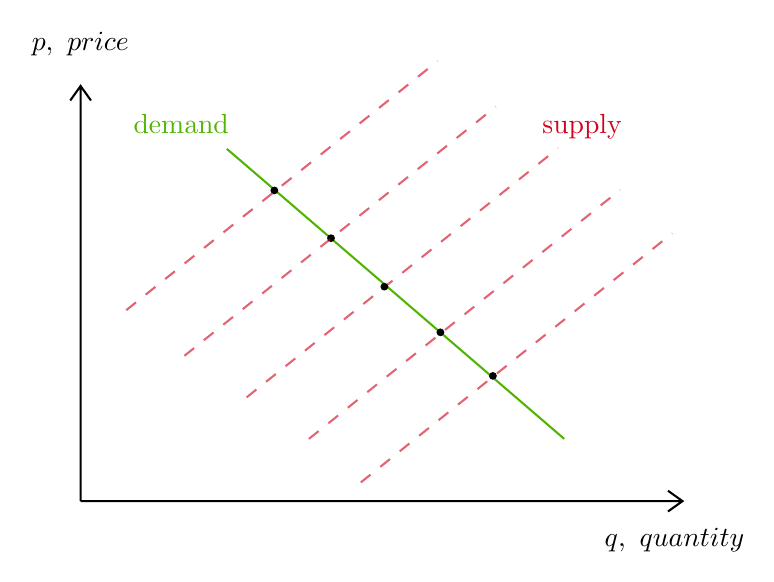
\begin{tikzpicture}[x=0.75pt,y=0.75pt,yscale=-1,xscale=1]
%uncomment if require: \path (0,416); %set diagram left start at 0, and has height of 416

%Shape: Axis 2D [id:dp7232537425646829] 
\draw  (160,270) -- (450,270)(160,70) -- (160,270) -- cycle (443,265) -- (450,270) -- (443,275) (155,77) -- (160,70) -- (165,77)  ;
%Straight Lines [id:da09936562819974382] 
\draw [color={rgb, 255:red, 81; green, 179; blue, 2 }  ,draw opacity=1 ]   (230.43,100.27) -- (242.29,110.44) -- (393,240) ;
%Straight Lines [id:da434828806821248] 
\draw [color={rgb, 255:red, 208; green, 2; blue, 27 }  ,draw opacity=0.61 ] [dash pattern={on 4.5pt off 4.5pt}]  (182,178) -- (332,58) ;
%Straight Lines [id:da7067480974690954] 
\draw [color={rgb, 255:red, 208; green, 2; blue, 27 }  ,draw opacity=0.61 ] [dash pattern={on 4.5pt off 4.5pt}]  (240,220) -- (390,100) ;
%Straight Lines [id:da6860399852947346] 
\draw [color={rgb, 255:red, 208; green, 2; blue, 27 }  ,draw opacity=0.61 ] [dash pattern={on 4.5pt off 4.5pt}]  (270,240) -- (420,120) ;
%Flowchart: Connector [id:dp6703726074956241] 
\draw  [fill={rgb, 255:red, 0; green, 0; blue, 0 }  ,fill opacity=1 ] (279.29,143.32) .. controls (279.29,142.59) and (279.89,142) .. (280.64,142) .. controls (281.39,142) and (282,142.59) .. (282,143.32) .. controls (282,144.05) and (281.39,144.64) .. (280.64,144.64) .. controls (279.89,144.64) and (279.29,144.05) .. (279.29,143.32) -- cycle ;
%Flowchart: Connector [id:dp42343723539931355] 
\draw  [fill={rgb, 255:red, 0; green, 0; blue, 0 }  ,fill opacity=1 ] (357.29,209.68) .. controls (357.29,208.95) and (357.89,208.36) .. (358.64,208.36) .. controls (359.39,208.36) and (360,208.95) .. (360,209.68) .. controls (360,210.41) and (359.39,211) .. (358.64,211) .. controls (357.89,211) and (357.29,210.41) .. (357.29,209.68) -- cycle ;
%Flowchart: Connector [id:dp3602533313351184] 
\draw  [fill={rgb, 255:red, 0; green, 0; blue, 0 }  ,fill opacity=1 ] (305,166.68) .. controls (305,165.95) and (305.61,165.36) .. (306.36,165.36) .. controls (307.11,165.36) and (307.71,165.95) .. (307.71,166.68) .. controls (307.71,167.41) and (307.11,168) .. (306.36,168) .. controls (305.61,168) and (305,167.41) .. (305,166.68) -- cycle ;
%Flowchart: Connector [id:dp5055341802748268] 
\draw  [fill={rgb, 255:red, 0; green, 0; blue, 0 }  ,fill opacity=1 ] (252,120.32) .. controls (252,119.59) and (252.61,119) .. (253.36,119) .. controls (254.11,119) and (254.71,119.59) .. (254.71,120.32) .. controls (254.71,121.05) and (254.11,121.64) .. (253.36,121.64) .. controls (252.61,121.64) and (252,121.05) .. (252,120.32) -- cycle ;
%Flowchart: Connector [id:dp7460489090675402] 
\draw  [fill={rgb, 255:red, 0; green, 0; blue, 0 }  ,fill opacity=1 ] (332,188.68) .. controls (332,187.95) and (332.61,187.36) .. (333.36,187.36) .. controls (334.11,187.36) and (334.71,187.95) .. (334.71,188.68) .. controls (334.71,189.41) and (334.11,190) .. (333.36,190) .. controls (332.61,190) and (332,189.41) .. (332,188.68) -- cycle ;
%Straight Lines [id:da27407798874237244] 
\draw [color={rgb, 255:red, 208; green, 2; blue, 27 }  ,draw opacity=0.61 ] [dash pattern={on 4.5pt off 4.5pt}]  (210,200) -- (360,80) ;
%Straight Lines [id:da6180788422321196] 
\draw [color={rgb, 255:red, 208; green, 2; blue, 27 }  ,draw opacity=0.61 ] [dash pattern={on 4.5pt off 4.5pt}]  (295,261) -- (445,141) ;

% Text Node
\draw (184,82) node [anchor=north west][inner sep=0.75pt]  [color={rgb, 255:red, 81; green, 179; blue, 2 }  ,opacity=1 ] [align=left] {demand};
% Text Node
\draw (381,82) node [anchor=north west][inner sep=0.75pt]  [color={rgb, 255:red, 81; green, 179; blue, 2 }  ,opacity=1 ] [align=left] {\textcolor[rgb]{0.82,0.01,0.11}{supply}};
% Text Node
\draw (135,42.4) node [anchor=north west][inner sep=0.75pt]    {$p,\ \text{price}$};
% Text Node
\draw (411,281.4) node [anchor=north west][inner sep=0.75pt]    {$q,\ \text{quantity}$};


\end{tikzpicture}
                \caption{Instrument shifting supply curve}
                \label{fig:endogeneity/sem/iv}
            \end{figure}
            

        \subsection{IV estimation}
            Since we have established that  is an instrumental variable, we can estimate  with IV. Recall the definition of the IV estimator:
            \begin{align}
                \hat\beta^{(s),IV}_1 = \frac{\ecov{z^{(s)},q}}{\ecov{z^{(s)},p}}
            \end{align}
            We can implement this in STATA by performing the 2SLS method,
            \begin{itemize}
                \item \textbf{First stage.} Estimate the regression
                \begin{align}
                    p_i = \pi_0 + \pi_1 z_i^{(s)} + e_i
                \end{align}
                and obtaining the estimate $\hat p_i = \hat\pi_0 + \hat\pi_1 z_i^{(s)}$.

                \item \textbf{Second stage.} Estimate the regression
                \begin{align}
                    q_i = \beta_0^{(d)} + \beta_1^{(d)} \hat p_i + u_i^{(d)}
                \end{align}
            \end{itemize}
            
            To implement in STATA, refer to the code in Lising \ref{lst:endogeneity/SEM/2SLS}.
            \begin{sexylisting}[colback=white, label=lst:endogeneity/SEM/2SLS]{2SLS SEM estimation}
ivregress 2sls qty (price = supply_shift), robust
            \end{sexylisting}

            
        \subsection{Reduced form estimation}

            We know that in equilibrium, demand is equal to supply, therefore setting \eqref{eq:endogeneity/demand} equal to \eqref{eq:endogeneity/supply_w_IV}, by 
            \begin{itemize}
                \item \textbf{equating} $q_i$, we obtain
                \begin{align}
                    \beta_0^{(d)} + \beta_1^{(d)}p_i + e_i^{(d)} = \beta_0^{(s)} + \beta_1^{(s)}p_i + \beta_2^{(s)}z^{(s)}_i + e_i^{(s)}
                \end{align}
                which rearranges to yield
                \begin{align}
                    p_i = \pi_0 + \pi_1 z_i^{(s)} + e_i
                \end{align}
                where
                \begin{align}
                    \delta_0 := \frac{\beta_0^{(s)} - \beta_0^{(d)}}{\beta_1^{(d)} - \beta_1^{(s)}},\quad \delta_1 := \frac{\beta_2^{(s)} - \beta_0^{(d)}}{\beta_1^{(d)} - \beta_1^{(s)}},\quad e_i := \frac{u_i^{(s)}-u_i^{(d)}}{\beta_1^{(d)} - \beta_1^{(s)}}
                \end{align}

                \item \textbf{equating} $p_i$ (first rearranging \eqref{eq:endogeneity/demand} and \eqref{eq:endogeneity/supply_w_IV} for $p_i$), it can be shown that 
                \begin{align}
                    q_i = \pi_0 +\pi_1 z_i^{(s)} + v_i
                \end{align}
                where
                \begin{align}
                    \pi_0 := \beta_0^{(d)},\quad\pi_1 := \frac{\beta_1^{(d)}\beta_2^{(s)}}{\beta_1^{(d)} - \beta_1^{(s)}},\quad v_i = \frac{\beta_1^{(d)}u_i^{(s)} - \beta_1^{(s)}u_i^{(d)}}{\beta_1^{(d)} - \beta_1^{(s)}}
                \end{align}
            \end{itemize}
            Therefore, we note that the ratio of the coefficients gives $\beta_1^{(d)}$, more precisely,
            \begin{align}
                \beta_1^{(d)} = \frac{\pi_1}{\delta_1}
            \end{align}
            There we have it - if we estimate the two reduced form equations, then we can estimate the demand curve slope.
